% !TEX TS-program = pdflatex
% !TEX encoding = UTF-8 Unicode
% !BIB TS-program = biber
% !BIB program = biber

\documentclass[12pt]{article}

%%% PAGE DIMENSIONS
\usepackage[margin=2.54cm]{geometry}
\geometry{a4paper} 
% \usepackage{caption}
% \usepackage{subcaption}
\usepackage{graphicx} % For better graphics
\usepackage{pdfpages} % To insert pdfs into the library
\usepackage{tikz}
\usepackage{wrapfig}
\usepackage{siunitx}
% Packages to add projects
\usepackage{movie15}
\usepackage{qtree}
% Display multiplication and division sums
\usepackage{xlop}
\usepackage{longdivision}

%%% PACKAGES
\usepackage{booktabs} % for much better looking tables
\usepackage{amsmath} % for better maths
\usepackage{paralist} % very flexible & customisable lists (eg. enumerate/itemize, etc.)
\usepackage{verbatim} % adds environment for commenting out blocks of text & for better verbatim
\usepackage{subfig} % make it possible to include more than one captioned figure/table in a single float
\usepackage[framed,numbered]{matlab-prettifier} % enable inserting matlab code.
\usepackage[parfill]{parskip}
%\addtolength{\jot}{1em}
\usepackage{amssymb}
\usepackage{cancel}
\usepackage{color}
\usepackage{listings}
% Create Listing Colours
\usepackage{xcolor}
% Create directory structures
\usepackage{dirtree}
% Enable landscape functionality
\usepackage{pdflscape}
% Enable the setspace package
\usepackage{setspace}
\doublespacing

% \definecolor{codegreen}{RGB}{0,255,0}
% \definecolor{codegray}{RGB}{105,105,105}
% \definecolor{codepurple}{RGB}{138,43,226}
% \definecolor{backcolour}{RGB}{255,255,255}
\definecolor{codegreen}{rgb}{0,0.6,0}
\definecolor{codegray}{rgb}{0.5,0.5,0.5}
\definecolor{codepurple}{rgb}{0.58,0,0.82}
\definecolor{backcolour}{rgb}{0.95,0.95,0.92}

\lstdefinestyle{mystyle}{
    backgroundcolor=\color{backcolour},   
    commentstyle=\color{codegreen},
    keywordstyle=\color{magenta},
    numberstyle=\tiny\color{codegray},
    stringstyle=\color{codepurple},
    basicstyle=\ttfamily\footnotesize,
    breakatwhitespace=false,         
    breaklines=true,                 
    captionpos=b,                    
    keepspaces=true,                 
    numbers=left,                    
    numbersep=5pt,                  
    showspaces=false,                
    showstringspaces=false,
    showtabs=false,                  
    tabsize=2
}
\lstset{style=mystyle}

\usepackage{multicol}
\usepackage{float}

% References
\usepackage[backend=biber,style = apa]{biblatex}
\bibliography{sources}

%%% HEADERS & FOOTERS
\usepackage{fancyhdr} % This should be set AFTER setting up the page geometry
\setlength{\headheight}{15pt}
\pagestyle{fancy} % options: empty , plain , fancy
\renewcommand{\headrulewidth}{0pt} % customise the layout...
\lhead{}\chead{}\rhead{}
\lfoot{}\cfoot{\thepage}\rfoot{}

%%% SECTION TITLE APPEARANCE
\usepackage{sectsty}

%%% ToC (table of contents) APPEARANCE
\usepackage[nottoc,notlof,notlot]{tocbibind} % Put the bibliography in the ToC
\usepackage[titles,subfigure]{tocloft} % Alter the style of the Table of Contents
\renewcommand{\cftsecfont}{\rmfamily\mdseries\upshape}
\renewcommand{\cftsecpagefont}{\rmfamily\mdseries\upshape} % No bold!

%%% Hyperlinking 
\usepackage{hyperref}
\begin{document}
\begin{titlepage}
	\newcommand{\HRule}{\rule{\linewidth}{0.5mm}} % Defines a new command for horizontal lines, change thickness here
	
	\center
	
	%------------------------------------------------
	%	Headings
	%------------------------------------------------
	
	\textsc{\LARGE }\\[1.5cm] % Main heading such as the name of your university/college
	
	\textsc{\Large Finance 705}\\[0.5cm] % Major heading such as course name
	
	%------------------------------------------------
	%	Title
	%------------------------------------------------
	
	\HRule\\[0.5cm]
	
	{\huge\bfseries Research Proposal: \\Data Science in Private Equity}\\[0.4cm] % Title of your document
	
	\HRule\\[0.5cm]
	
	%------------------------------------------------
	%	Author(s)
	%------------------------------------------------
	
	{\large\textit{Connor Robert McDowall}}\\

	%------------------------------------------------
	%	Date
	%------------------------------------------------
	
	\vfill\vfill\vfill % Position the date 3/4 down the remaining page
	
	{\large\today} % Date, change the \today to a set date if you want to be precise
	 
	%----------------------------------------------------------------------------------------
	
	\vfill % Push the date up 1/4 of the remaining page
	
\end{titlepage}
\pagenumbering{roman}
\section{Abstract}
This research proposal aims to validate and extend the contributions made by Block et al (\citeyear{BLOCK2019329}). 
They identify seven investment criteria crucial for investment decision making in private equity. 
We explore if data science can improve screening efficiency in investment due diligence for private equity fund managers when assessing investment and exit opportunities. 
We propose forming numeral and categorical proxies for the investment criteria from private company data stored in PitchBook. 
Subsequently, we propose the implementation of the data science process proposed by Aur{\'e}lien G{\'e}ron (\citeyear{aurelien2017hands}).
We will train three supervised learning algorithms to make predictions on investment/exit opportunities. 
These models are Multi-nominal Logistic Regressions, Random Forests, Multi Layer Perceptrons (MLP).
The proposed contributions aim to validate the investment criteria, validate the use of PitchBook for research purposes, and show evidence data science can inform investment due diligence and create efficiencies in screening for investments.
\newpage
\tableofcontents
\listoffigures
\listoftables
\newpage
\pagenumbering{arabic}
\section{Introduction}\label{intro}
Private Equity (PE) is an alternative asset class with similar characteristics to hedge funds.
Private equity funds are investment vehicles usually identified by four characteristics. 
Firstly, they are privately organized, pooling capital from several parties.
Secondly, professional investment managers administer the fund. Their incentives are performance-based including compensation and significant carry in the fund.
Thirdly, they are inaccessible to the public.
Lastly, they operate externally to securities regulation and registration requirements.
A private equity fund is managed by general partners (GP) who manage limited partners' (LP) investments in the fund. 
LPs make passive investments with little to no control in the fund's operations. 
Private equity funds typically charge a 2\% annual fee and 20\% performance fee on the fund's annual return.
They raise capital through private offerings and pursue investment strategies in private markets based on the funds mandate to generate returns for investors (\cite{brav2008hedge}).
Data science combines scientific methods, maths, statistics, specialized programming, advanced analytics, AI, and even storytelling to uncover and explain the business insights buried in data (\cite{IBM}).
The number of data science applications are increasing in most industries but there is slow uptake in private equity. 
This creates opportunities to use emerging technologies to add value in operational and investment processes, 
exemplified through case studies featuring BCG (\citeyear{BCG}), Blackstone (\citeyear{BBBS}) and the NZ Super Fund.
Section \ref{lit-review} evaluates the prior literature related to private equity and decision processes by fund managers.
Section \ref{Hyp-dev} frames hypotheses to extend the contributions by Block et al (\citeyear{BLOCK2019329}).
In particular, this section explores if data science can improve screening efficiency in investment due diligence for private equity fund managers when assessing investment opportunities?
Section \ref{data} outlines the variables of interests with investment criteria and investment decision/exit opportunities, the dependent and independent variables respectively.
Furthermore, explanations outline the derivation of investment criteria from the database PitchBook, limitations with the database, and contingency plans on the provision of poor quality data from PitchBook.
Section \ref{methods} conveys how this research proposal will follow conventional data science processes proposed by Aur{\'e}lien G{\'e}ron (\citeyear{aurelien2017hands}), and implement the three forms of supervised learning algorithms:
Multi-nominal Logistic Regression, Random Forests, and Multi-Layer Perceptrons.
Section \ref{conclusions} concludes with the key contributions and a few suggestions for future research.
\section{Literature Review}\label{lit-review}
Prior literature emphasizes generated returns, comparisons to public markets, and value created from private equity.
The presence of cyclicality in PE returns differs according to fund type and is consistent with the conjecture that capital market segmentation contributes to private equity returns (\cite{cavagnaro2019measuring}).
Institutional investors returns are not from chance alone, but skill leads to outperformance when selecting private equity investors (\cite{ang2018estimating}).
The adaptation of stochastic discount factor valuation methods to evaluate performance for venture capital generalized the Popular Market Equivalent (PME) method to reflect risk-free rates and public returns found abnormal performance (\cite{korteweg2016risk}).
Evidence of differences in skill and exit styles among venture partners investing at the same VC firm at the same time estimates human capital is two to five times more important than a VC firm’s organizational capital in explaining performance (\cite{ewens2015vc}).
Classification of risks and post-investment actions inform agency and hold-up problems are important to contract design and monitoring (\cite{kaplan2004characteristics}).
The analysis of firm and VC characteristics, in combination with value-increasing investments post-IPO for both VC’s and underlying companies, is an efficient solution to information problems (\cite{iliev2020venturing}).
Harris et al (\citeyear{harris2014private}) found buyout performance consistently exceeds the public markets (S\&P 500) by 3\% annually, calculated using the Burgiss data set. 
The performance in Cambridge Associates and Preqin datasets is qualitatively consistent with Burgiss but lower in Venture Economics.
The determinant of leverage in buyouts is variation in economy-wide credit conditions. 
Higher deal leverage is associated with higher transaction prices and lower buyout fund returns.
This suggests that acquirers overpay when access to credit is easier (\cite{axelson2013borrow}).
Investments in innovation, measured by patenting activity, informs one form of long-run activity. 
Based on 472 LBO transactions, there is no evidence that LBOs sacrifice long-term investments (\cite{lerner2011long}).
Phalippou (\citeyear{phalippou2020inconvenient}) finds evidence private equity performance does not exceed public markets after considering carry and other factors.
The above literature eludes to the presence of multiple factors and investment criteria when making investment decisions.
Block et al (\citeyear{BLOCK2019329}) explore investment criteria with an experimental conjoint analysis of private equity fund-types to inform how investments are made.
There has been a comprehensive investigation on the effects of PE financing in corporate and entrepreneurial finance.
Empirical analysis in precedent literature finds evidence of improvements to operating performance from PE investment (\cite{kaplan2009leveraged}) and public market outperformance ((\cite{ang2018estimating}),(\cite{braun2017persistent}), (\cite{harris2014private}), (\cite{kaplan2005private}), (\cite{kaplan2015private}), (\cite{phalippou2009performance}), (\cite{robinson2013private})).
The exploration of PE investments across fund types and size yield consistent results ((\cite{kaplan1989effects}), (\cite{chemmanur2011does})).
Selection and treatment effects ascribe to increased performance ((\cite{bengtsson2011investor}), (\cite{bernstein2016impact}), (\cite{RIN2013573}), (\cite{LCVC})).
The active investment nature of PE enables portfolio companies the provision of value-added activities, either direct or indirect.
Direct benefits include access to coaching or networks. 
Indirect benefits include certification effects to third parties ((\cite{BOTTAZZI2008488}), (\cite{gompers2001venture}), (\cite{hellmann2002venture}), (\cite{korteweg2017skill}), (\cite{lerner1995venture})).
Portfolio company selection, and the capacity to add value through financial, governance and operational engineering, are the skillsets emphasized by PE investors. 
Contrary to the importance of investment selection, there is very little literature exploring investment selection and decision making by private equity managers.
PE managers expend considerable resources in evaluating and screening investment opportunities ((\cite{kaplan2001venture}), (\cite{gompers2016private})).
Their investment screening and selection process reviews many companies while only investing in a select few.
Gompers et al (\cite{gompers2016private}) reports for every hundred investment opportunities, the average PE investor conducts thorough due diligence on 15, 
enters agreements with eight, and eventually closes fewer than four. 
Empirical challenges associated with isolating the effect of different company characteristics contribute to the lack of empirical evidence surrounding investment criteria.
Block et al (\citeyear{BLOCK2019329}) are one of the first groups to investigate the investment criteria of PE investors, given decision making in PE is often debated ((\cite{gompers2001venture}), (\cite{kaplan2004characteristics})).
The use of observational data is not feasible as observing investor preferences between two identical companies that vary in predetermined characteristics is not possible.
Adopting similar methodologies to Bernstein et al (\citeyear{bernstein2017attracting}), Block et al (\citeyear{BLOCK2019329}) compares 
decision making across different investor types using a large-scale conjoint analysis of 19,474 screening decisions by 749 PE investors
through contacting 15,600 investment professionals listed in PitchBook. 
The conjoint analysis enables a more accurate representation of actual decision making as captures decisions making trade offs between criteria.
Block et al (\citeyear{BLOCK2019329}) required participants to make a series of assessments on a set of discrete company attributes. 
In particular, these attributes are: (1) profitability, (2) revenue growth, (3) track record of management team, (4) reputation of current investors, (5) business model, (6) value-added of product/service, and (7) international scalability.
Every participant needed to evaluate multiple companies which differ only in the specifications of the above attributes and recommend investment decisions.
A multi-level logistic regression model evaluated and compared the importance of different investment criteria, enabling criteria comparisons across investor types.
Lerner et al (\cite{lerner2007smart}) identifies there are likely differences in decision making between investor types with a broader perspective on investing behaviour underdeveloped (\cite{hellmann2013angels}).
Block et al (\citeyear{BLOCK2019329}) investigates analysis with greater granularity to explore decisions by different investor types. 
In particular, investor types explored in this analysis are, (1) family offices, (2) business angels, (3) venture capital funds, (4) growth equity funds, and (5) leveraged buyout funds.
Firstly, Block et al (\citeyear{BLOCK2019329}) identify the relative importance of PE investors' investment criteria.
In order of importance, revenue growth, value-added (product/service), and management team track record are the most important criteria.
Internationally scalability, current profitability, business model, and reputation of existing investors are relevant but of lower importance.
Secondly, Block et al (\citeyear{BLOCK2019329}) compare the importance of the respective investment criteria across different investor types.
They provide systematic empirical comparison methods of these differences and find family offices, growth equity funds and leveraged buyout funds prefer profitability over revenue growth. 
Venture capital funds and business angels prefer revenue growth over profitability.
These findings imply discrepancies in the risk profiles between investor types.
In the case of family offices, the results align with the objective of a family office to preserve wealth in order to maintain financial and social standing.
The above literature informs the investment criteria to considered when evaluating investment decisions in PE.
\section{Hypotheses Development}\label{Hyp-dev}
\subsection{Research Question}
This research proposal aims to extend the contributions from Block et al (\citeyear{BLOCK2019329}).
Gompers et al (\cite{gompers2016private}) inform the closure of fewer than four out of hundred investment opportunities.
The wrong investment decisions may have serious consequences for both fund returns and manager reputation.
Kaplan et al (\citeyear{kaplan2001venture}) and Gompers et al (\citeyear{gompers2016private}) reiterate PE managers expend considerable resources evaluating and screening investment opportunities.
Block et al (\citeyear{BLOCK2019329}) identified several investment criteria integral to investment decisions: 
(1) profitability, (2) revenue growth, (3) track record of management team, (4) reputation of current investors, (5) business model, (6) value-added of product/service, and (7) international scalability.
Data science can automate manual processes and make predictions considering complex interactions between numerical and categorical variables.
Data science methodologies considering the variables proposed by Block et al (\citeyear{BLOCK2019329}), after surveying PE managers and their risk profiles,
may reduce screening time, reduce due diligence costs, and identify profitable investments aligning with investment mandates.
Subsequently, this research proposal will explore:
\begin{center}
	\textbf{Can data science improve screening efficiency in investment due diligence for private equity fund managers when assessing investment opportunities?}
\end{center}
In layman's terms, improving screening efficiency relates to accurately predicting suitable companies to invest.
This process supports company selection when using traditional screening processes and considers the investment criteria proposed by Block et al (\citeyear{BLOCK2019329}).
Depending on the success of screening models, these practices may replace existing screening methods, adding value to both investment due diligence processes and PE fund managers.
\subsection{Hypotheses}
The proposition of the below hypotheses aims to investigate the research question:
\begin{align}
	H_0:& \text{ Data science models do not predict suitable investment targets.}\\
	H_1:& \text{ Data science models do predict suitable investment targets.}
\end{align}
Suitable investment targets are companies that either currently, or are predicted to, align with Block et al (\citeyear{BLOCK2019329}).
Data science methodologies will also test if the investment criteria proposed by Block et al (\citeyear{BLOCK2019329}) after surveying PE managers identify suitable investment targets
and/or if there are other unexplained contributing factors/interactions.
\section{Data}\label{data}
\subsection{Variables: Inputs}\label{var}
Block et al (\citeyear{BLOCK2019329}) implemented a two-step process to evaluate the screening criteria.
Firstly, prior research informs an investment criteria long-list ((\cite{bernstein2017attracting}), (\cite{VCEST}), (\cite{LCVC})).
Secondly, Block et al (\citeyear{BLOCK2019329}) conducted 19 expert interviews with PE investors across Europe and the US, identifying the most relevant criteria
After their analysis, they discovered the relative importance of PE investors' investment criteria across multiple investor types.
These criteria are, (1) profitability, (2) revenue growth, (3) track record of management team, (4) reputation of current investors, (5) business model, (6) value-added of product/service, and (7) international scalability.
One must highlight the definition of business models comes from Amit et al (\citeyear{Amit2001493}).
Block et al (\citeyear{BLOCK2019329}) outlined the attributes and attribute levels for the above investment criteria, used in the conjoint analysis, in figure \ref{fig:ica}.
The following subsections include the descriptions of these attributes (figure \ref{fig:ica}).
This proposition aims to explore these criteria paired with common financial, operational and categorical variables displayed in table \ref{table:1}.
\subsubsection{Revenue Growth}
Revenue growth describes the average yearly revenue growth over the last years. 
This is a categorical variable with four designations: 10\% p.a., 20\%p.a., 50\%p.a., and 100\%p.a. 
These growth rates will be considered over one, three and five year time periods, assigned to the closest category.
Additionally, revenue growth will be included as a numerical variable for comparison purposes. 
\subsubsection{Value-added (Product/Service)}
Value-added services (product/services) describes the value added to the customer from the product or service.
Low value represents a marginal improvement (e.g., cost reduction or service quality), whereas high value represents significant improvements.
This is a categorical variable with three designations: low, medium, and high.
Value-added is a difficult variable to measure. 
However, using sentiment analysis with Natural Language Processing (\cite{NLP}) with non-financial data (e.g. social media mentions, web traffic, news features and reviews) 
would enable the categorization of value-added services.
\subsubsection{Management Team Track Record}
Management team track record describes whether the management team has a relevant track record (e.g. industry and leadership experience).
This is a categorical variable with three designations: none of them, some of them, all of them.
Multi-nominal logistic regression will consider executive experience and education to create the above categorical variables (\cite{EDGAR201795}).
\subsubsection{International Scalability}
International scalability describes the difficulty of scaling internationally, in terms of the time and investments needed.
This is a categorical variable with three designations: easy, medium and difficult.
Multi-nominal logistic regression will consider various features (e.g., industry classification, committed capital, market presence, years since founding etc.) to create the required categorical variables (\cite{EDGAR201795}).
\subsubsection{Profitability}
Profitability describes the current profitability of the company, a categorical variable with three designations: not profitable, breakeven, and profitable.
Multi-nominal logistic regressions will consider the following financial values to form the above categorical variables: 
Earnings Before Interest, Tax, Depreciation and Amortization (EBITDA); 
Earnings Before Interest and Tax(EBIT);
Net Operating Performance After Tax (NOPAT);
Return on Assets (ROA);
and Return on Equity (ROE).
Additionally, EBIT, EBITDA, NOPAT, ROA, and ROE will be included as numerical variables for comparison.
\subsubsection{Business Model}
Business model describes the key focus of the company based on prior research (\cite{Amit2001493}) pertaining to four designations: (1) Lock-in, (2) Innovation-centered, (3) Low cost, and (4) Complimentary.
The Lock-in model keeps customers attracted and 'locked in', having high switching costs for customers, which prevent them from changing to other providers.
The Innovation-centered model offers innovation in the form of new technology, products or services.
The Low cost model focusses on reducing costs for customers for already existing products or services.
The Complimentary model bundles multiple goods and services to generate more value for customers.
This is also a difficult variable to derive.
Business descriptions would be input into the text classification functionalities in Natural Language Processing (\cite{NLP}) to categorize models designations.
This will be difficult.
\subsubsection{Current Investors}
Current investors describes the types of investors, if any.
This is a categorical variable with three designations: no other current external investors, other current external investors - unfamiliar, and other current external investor - Tier 1.
Tier 1 investors are reputable investors.
Investor relationships can be modelled using the mathematics behind graph theory and network analysis from geographical applications ((\cite{CURTIN2018153}), (\cite{FAUDREE200315})).
Modelling the strength in investor relationships and investment history, in combination with multi-nominal logistic regression analysis, will categorize the necessary designations.
However, this will also be difficult.
\subsubsection{Year}
The consideration of a yearly designation (e.g., 2016, 2017 etc.) related to the collection of investment criteria proposed by Block et al (\citeyear{BLOCK2019329}) will inform time-series analysis.
\subsection{Variable: Output(s)}
Block et al (\citeyear{BLOCK2019329}) explored the importance of investment criteria through multi-level logistic regressions models.
The investment decision is binary: 0 if no investment, 1 if investment. Multi-level logistic regressions account for both nested investment decisions and multi-level effects.
This proposal will explore a similar outcome of an investment decision (0 if no investment, 1 if investment).
Additionally, the exploration of three exit outcomes based on investment criteria will contribute to the validation of an investment target.
These outcomes are, (1) IPO, (2) Acquisition, and (3) Bankruptcy/failure.
In lyman's terms, identify the likely exit outcomes and suitable time to exit a company for a PE manager.
Ross et al (\citeyear{ross2021capitalvx}) explore this phenomena with models trained on a different set of features using a different dataset (\cite{CB}).
The inclusion of the desired outcomes in the datasets enables the most appropriate algorithms for this proposal (Section \ref{algorithms}).
It must be highlighted their findings are not published in top ranked journal, they don't consider key financial or operation variables in their feature selection,
and lacks rigorous comparisons to traditional empirical methods (e.g., logistic regressions) to cross-validate results. It is poor quality research.
This research proposal will explore the above exit outcomes using investment criteria considered by PE investors and cross-validate results with logistic regressions where possible.
\subsection{Sources}
\subsubsection{PitchBook}
PitchBook is financial data and software company that provides thousands of professional's comprehensive data on private and public market information (\cite{PB}).
Block et al (\citeyear{BLOCK2019329}) identifies PitchBook as one of the most comprehensive databases in entrepreneurial finance, regularly used for PE related research ((\cite{kaplan2016venture}),(\cite{PAGLIA2014177})).
Disclosed information from limited partners, filings of national regulators and other available information are the main contributors to the database.
PitchBook has advantages over alternative databases as reports information on investment teams and contact details in addition to information on the investment entity (\cite{brown2015different}).
The database records comprehensive data on companies, investors, deals, M\&A, LPs, funds, financials, advisors, professionals, debt \& lenders.
In particular:
\begin{itemize}
	\item Companies of various designations (Publicly traded, Pre-IPO, PE-backed, Startups/Stealth etc.)
	\item Deal information (Bankruptcies, IPOs, PIPEs, LBO, VC Investments etc.)
	\item Financial information (calculation transparency, balance sheets, cash flow statements, income statements, consensus information, deal multiples, financial ratios, fundamentals etc.)
\end{itemize}
Data, both time-series and cross-sectional, is accessible using application programming interfaces (API) or direct downloads to excel formats (e.g., xlsx etc.)
Industry widely adopt the platform as the product has high levels of granularity for data science applications.
PitchBook continues to grow as industry and PitchBook employees continue to contribute to the platform.
An itemized illustration, of the size and scope of available data, as at 03/06/2021 follows:
\begin{enumerate}
	\item \textbf{Deals}: 1,540,549 deals with 45 deals types, evaluate deal histories, get key information and deal multiples, access pre and post money valuations, explore series terms and stock information.
	\item \textbf{Companies}: 3,096,933 (private), 58,362 (public), get key information, explore financing history, evaluate financials and filings, view executives and board members, follow non-financial metrics.
	\item \textbf{Financials}: Financials and estimates summary, analyse key metrics, explore balance sheets, income statements, cash flows, ratios \& multiples.
\end{enumerate}
PitchBook is an appropriate data source as Block et al (\citeyear{BLOCK2019329}) surveyed investors from this database,
and it provides all the information required to derive the set of variables described in Section \ref{var}.
\subsection{Limitations: PitchBook}
The main contributors to PitchBook are disclosed information from limited partners, filings from national regulators and other publicly available information.
Additionally, there is self-selection bias as private companies elect to disclose information-related to their companies.
This research proposal is unable to provide descriptive statistics on the data available from PitchBook as requires a service subscription.
The derivation of Business Model and Value-added categorical variables will be difficult as require an implementation of a complex algorithm.
However, it is feasible.
The aforementioned limitations may create poor quality datasets when taking global perspectives. 
This research proposal will focus on the North American market in an attempt to minimize data issues as data pertaining to this market is the most complete.
If the data is unsuitable for analysis after these considerations, we will explore the alternative datasets and sources in Section \ref{ADS}.
\subsection{Alternative Data Sources}\label{ADS}
The consideration of alternative data sources will form contingency plans if data issues persist with PitchBook.
A consortium of databases is necessary to construct the variables of interest described in 
MergerMarket (\citeyear{MM}) and CB Insights (\citeyear{CBI}) have a comprehensive M\&A database on relevant deals.
Crunchbase (\citeyear{CB}) contain investment professional, identification and non-financial information on early stage companies.
Preqin (\citeyear{PQ}) includes comprehensive information on PE managers.
In addition to the above databases, liaising and partnering with local and global PE managers may help source the required data to create variables.
However, PitchBook is more comprehensive than the consortium of alternatives as contains all the  required information for investment criteria variable construction.
The research proposal may be put on hold until better quality data comes to market on the basis both PitchBook and the consortium of alternatives fail to provide the required data.
\section{Methodology}\label{methods}
The research methodology will follow the conventional data science process proposed by Aur{\'e}lien G{\'e}ron (\citeyear{aurelien2017hands}). 
This process is: 
(1) Get the “Big picture”. 
(2) Get the Data. 
(3) Discovery \& Visualization. 
(4) Data Preparation.
(5) Model Selection \& Training.
(6) Model Tuning.
(7) Presentation.
(8) Launch, Monitor, and Maintain System (Omitted).
We explore each step sequentially from Section \ref{method-prob-solv} to Section \ref{method-launch}.
and highlight the mathematics pertaining to the methodology is listed in the Appendix (Section \ref{math}).
\subsection{Problem Scoping} \label{method-prob-solv}
\subsubsection{Problem Framing}
Problem scoping involves three processes: framing the problem, selecting performance measures, and checking data assumptions.
Sections \ref{intro}, \ref{lit-review} and \ref{Hyp-dev} frame the objective of this research proposal.
Currently no other solutions or prior literature on using the investment criteria proposed by Block et al (\citeyear{BLOCK2019329}) exist
to train data science models with the objective of informing and increasing the efficiency of investment screening and selection for PE fund managers.
\subsubsection{Performance Measure Selection} \label{perf-meas}
Performance measures evaluate the accuracy of machine learning models to validate predictions.
The computation of Root Mean Square Error (RMSE) and Mean Absolute Error (MAE) will inform predictability.
Both are cost functions and measure the distance between vectors.
RMSE calculates the standard deviation of errors between the observed values ($y^{(i)}$) and values predicted by the model ($h(\textbf{x}^{(i)}$). 
This performance measure is the preferred the algorithms discussed in Section \ref{algorithms}.
The number of instances in the dataset (m) is comparable to a datapoint with combinations of time-series and cross-sectional data in conventional empirical datasets.
$\textbf{x}^{(i)})$ is a vector of all feature values for the ith instance.
In layman's terms, the investment criteria (feature values) are described in Section \ref{data} for the ith company (instance).
\subsubsection{Checking Data Assumptions}
This research proposal builds on the investigation Block et al (\citeyear{BLOCK2019329}).
The numerical and categorical variables suggested in \ref{data} are appropriate. 
The outcomes of this research will inform an end-to-end methodology that do not rely on other systems or processes.
Addressing the data limitations in Section \ref{data} enable the implementation of this research proposal.
\subsection{Data Acquisition}
Firstly, there will be an initialization of a research workspace using the technologies itemized in the Appendix (\ref{tech}) and best practise proposed by Wilson et al (\citeyear{Wilson}).
The workspace enables a Python implementation, distributed by Anaconda, using several core modules: Numpy, Pandas, Matplotlib, Scikit-learn, and Tensorflow.
Microsoft Visual Code (IDE), complete with Git functionalities, will facilitate software development.
The hardware in use will be a MacBook Pro (2019) with macOS Mojave as the chosen operating system.
The use of IBM Watson and AWS technologies depends on hardware capabilities and the computational complexity of this methodology.
PitchBook, a subscription-based product, will provide the raw data pertaining to private companies.
Subsequently, collaboration with subscription holders is necessary.
A screening for US companies sorts US company-related information into one data source.
This sheet contains the relevant information to derive the required numerical and categorical investment criteria.
Downloading the results from the screening grants access to the data.
This is the matrix for feature values for all instances.
PitchBook grows iteratively as there are over 3 million private companies registered on the database.
It is important to automate a data pipeline to retrain models and provide up to date information.
This will be accomplished through controlling PitchBook's excel application programming interface (API) with a custom python module.
If the above data limitations related to PitchBook persist, 
industry collaboration enables the access to relevant data from their internal and external sources.
Additionally, the division of the feature matrix (\textbf{X}) into 
three sets is necessary to mitigate bias in both model selection and data snooping.
Random sampling will form three subsets: training, validation and testing respectively.
\subsection{Discovery \& Visualization}
Following on from data acquisition, it is important to get a general understanding of the data prior to manipulation and preparation.
Exploratory analysis will take place on the training set investigating a number of features pertaining to the dataset.
This analysis will explore geographical visualizations per US State to show concentrations of private entities,
correlations between numerical and categorical variables pertaining to unprocessed investment criteria
and explore the correlations between combinations of numerical and categorical variables.
\subsection{Data Preparation}\label{data-prep}
A series of transformation functions will be written for reproducibility on updated datasets and test variation in data transformations.
This will take the form of a transformation pipeline to apply to the training set feature matrix (\textbf{X}).
The pipeline will first incorporate cleansing functionalities to: remove missing variables, 
isolate the required variables in the feature matrix in order to derive investment criteria in Section \ref{data},
Numerical revenue and profitability values are converted to the designated categorical investment criteria proposed by Block et al (\citeyear{BLOCK2019329}).
Value-added (Product/Service) and Business Model categorical variables will require Natural Language Processing techniques to derive the attribute levels within these investment criteria.
The use of sentiment analysis with non-financial data (Section \ref{data}) using Tensorflow's Word2Vec \& Seq2Seq tutorials will derive Value-added (Product/Services) categories.
The use of NLP's text classification functionalities with company descriptions (Section \ref{data}) will categorize business models.
Variations in generalized multi-level logistic regressions (Section \ref{mllr-math}) using the relevant data to the desired investment criteria (Section \ref{data}) will categorize the variables needed for International Scalability, Management Team Track Record and Current Investors investment criteria.
The categorization of desired outcomes (outputs) for screening processes (investments and exits) will be binary (1 for each of a present outcome (investment, IPO, acquisition,  bankruptcy/failure), 0 otherwise). 
After, missing variables will be filled with median values on a case-by-case basis in order to include critical instances.
Thirdly, the transformation pipeline will convert text and categorical attributes to numerical values stored as SCiPy sparse matrices using scikit-learn's OneHotEncoder function.
Lastly, the transformation pipeline will implement feature scaling to rescale all input attributes to the same scale using scikit-learn's StandardScaler function.
Standardization subtracts the mean value and divides by the variance so the resulting distribution has unit variance.
This procedure does not bound values to a specific range (unlike normalization) but is much less affected by outliers.
Rescaling is required to optimize algorithm performance.
\subsection{Model Selection \& Training} \label{algorithms}
Data preparation is the most difficult section of the methodology.
Methods become elementary (my dear Watson) after data preparation.
Machine learning methods have a reputation for being 'blackboxes' with decision making opaque to users.
This generally creates adoption issues which may extend to PE managers given the lack of understanding in how the algorithms function.
Subsequently, this research proposal suggests three supervised learning, model-based methodologies: (1) Multi-nominal Logistic Regression, (2) Random Forests, and (3) Multi Layer Perceptrons (MLP).
Supervised machine learning algorithms include desired outcomes (labels) in the training sets and are the most transparent to PE managers e.g., these investment criteria contribute to this investment or exit decision.
These models enable predictions across both time-series and cross-sectional contexts.
These algorithm require nested mathematical functions.
We include their expression in the Appendix (\ref{math}).
\subsubsection{Multi-nominal Logistic Regression (Softmax Regression)} \ref{mllr-math}
Logistic regression estimates the probability that an instance belongs to a particular class.
This research proposal will consider the investment criteria of each instance to determine the probability of investment and exit outcomes.
The use of this algorithm is intuitive as enables cross-validation with the logistic regressions performed by Block et al (\citeyear{BLOCK2019329}).
This proposal suggests using two multi-nominal logistic regression, generalizations to support one investment decision and three exit outcomes respectively.
This algorithm computes a score, then estimates the probability of each class by applying the normalised exponential.
After calculating the scores for every class for the instance \textbf{x}, the probability $\hat{p}_{k}$ that the instance belongs to class k is calculated by running the scores 
through a softmax function. This function computes the exponential of every score then normalizes them.
The softmax regression classifier predicts the class with the highest estimate probability.
The models aims to estimate a high probability for the target class (and low probabilities for the other classes) through the minimization of a cross entropy cost function.
The computation of a gradient vector from the cross entropy cost function enables optimisation techniques, in this instance gradient descent, to find the parameter matrix $\Theta$ that minimizes the cost function.
Therefore the investment or exit decision.
Sckit-learn's LogisticRegression function applies this algorithm with the equation pertaining to the method in the Appendix (\label{mnlr-sr-math}).
\subsubsection{Random Forests}
The second algorithm is a Random Forest, an ensemble of decision trees.
Decision trees are an algorithm suitable for classification tasks.
They make predictions based on a branching structure and are relatively simple.
This research proposal suggests decision trees can estimate the probability an instance (company) 
belongs to a particular investment decision or exit opportunity.
Estimation starts at the root node. Each node explores two outcomes e.g., revenue growth is less than 20\% p.a. or 20\% and greater.
The algorithm will divide the training instances based on the binary criteria. 
A node will have three attributes: (1) samples, (2) value, and (3) gini.
Sample counts how many instances the node applies to e.g, 100,000 companies.
Value informs the number of instances per class applies to the node e.g, 40,000 invested, 60,000 not invested.
Gini is an impurity measure with purity (gini = 0) representing all training instances it applies to belong to the same class.
There are two forms of impurity measure: gini and entropy. Decisions at nodes form boundaries, forming partitions of instance groupings.
Decision trees can continue to form new nodes based investment criteria until it settles on the max depth or each leaf node is 'pure'.
Subsequently, a decision tree can estimate the probability that an instance belongs to an investment decision or exit opportunity.
Firstly, it traverses the tree to find the leaf node for this instance, then returns the ratio of training instances of class k in this node.
Requesting a prediction will return the class with the highest probability at this node. 
The Classification And Regression Training (CART) algorithm trains the decision trees.
Firstly, it splits the training set in two subsets using a single feature k and threshold $t_k$, searching for the pair producing the purest subsets (weighted by their size).
This process is recursive until either the user-defined max depth is reached or there are no further splits that will reduce impurity.
The 'optimal solution' is difficult to find as the optimal tree is a NP-Complete problem, requiring O(exp(m)) time causing intractability for fairly small trees.
Gini impurity measures leads to faster computations but entropy measures tend to produce more balanced tree.
Random forests are ensembles of decisions trees, combining combinations of decision trees trained using the same training algorithms with varying subsets of the training data.
This process forms a diverse set of classifiers with predictions, when aggregated, 
This proposal suggests using Scikit-learn's RandomForestClassifier to implement ensembles of decisions trees, applying the above process, to compute the equations in the Appendix (\ref{rf-math}).
Random forests are the most appropriate for PE-related decision making as they are the most intuitive and transparent of the three proposed supervised machine learning algorithms.
\subsubsection{Multi Layer Perceptron (MLP)}
Artificial Neural Nets (ANN) are versatile, powerful, and scalable.
They sit at the heart of deep learning as frequently outperform other machine learning algorithms on large and complex problems.
This research proposal suggests implementing two sets of multi-layer perceptron, a form of ANN, to predict investment decisions and exit opportunities from investment criteria.
A linear threshold unit (LTU) feeds the weighted sum of input values ($z=\textbf{w}^{T} \cdot \textbf{x}$) into a step function ($h_{w}(\textbf{x})=step(z)$).
A perceptron is a single layer of LTUs where each LTU is connected to every input.
Perceptrons are suitable for classification as output the positive investment decision or exit opportunity if a threshold is met.
Perceptrons utilize a training algorithm assessing the strength of connections between perceptrons while considering errors.
A perceptron is fed one training instance at a time, making predictions for each instance.
For every output LTU that produced a wrong prediction, it re-enforces the connection weights using the perception learning rule (Appendix (\ref{mlp-math})) from the inputs that would have contributed to the right prediction.
A Multi Layer Perceptron is composed of one LTU input layer, multiple LTU hidden layers and an output LTU layer.
The step functions in each LTU are replaced by a logistic or ReLU function ($\sigma(z)=\frac{1}{1+ exp(-z)}$ or $ReLU(z) = max(0,z)$ respectively) to enable gradient descent for optimisation.
A shared softmax function replaces the individual activation functions in the output layer to enable exclusive classification.
In this instance, the classification of investment decisions, or exit opportunties, from investment criteria.
Tensorflow's DNNClassifier function facilitates the implementation of MLPs in this proposal.
\subsubsection{Evaluation}
This proposal will utilise performance measures outlined in Section \ref{perf-meas} and cross-validation techniques with validation sets to inform the prediction proposed models.
Transparency decreases and complexity increases with Random Forests, Multi-nominal Logistic Regression and Multi Layer Perceptrons (MLP) respectively.
\subsection{Model Tuning}
Each model has a set of hyper parameters integral to performance. 
This proposal will conduct grid search, randomized search, error analysis and evaluations using test sets to find the best combination of hyper parameters to optimise model performance.
\subsection{Solution Presentation} \label{method-launch}
This research proposal will inform the feasibility of data science applications in private equity to assist with investment screening due diligence.
The above methodology will be converted to a custom python package distributed on the open-source Python Package Index (\citeyear{PYPL_Pop}) 
containing source code, package documentation, this research proposal, accompanying dissertation and technical guides to inform proposed algorithms.
Lastly, demonstrations will be made to private equity managers.
\section{Conclusions}\label{conclusions}
\subsection{Contributions}
This proposal is a very difficult to implement but has the potential to add tremendous value to investment screening and due diligence.
There are three key contributions in this research proposal:
Firstly, this proposal aims to validate the investment decision criteria proposed by surveyed PE managers gathered by Block et al (\citeyear{BLOCK2019329}).
Secondly, support arguments on PitchBook being a suitable database for future empirical research, especially with intersections between data science and private equity.
Lastly, provide evidence to PE managers data science can inform investment due diligence and create efficiencies in screening for investments.
\subsection{Future Research}
There are several new avenues for research depending on a successive outcome(s) from this proposal.
Firstly, this proposal only considers relative performance of investment criteria from the perspective of the average PE investor.
Further research could explore the segmentation of PE investor types (family office, business angel, venture capital, growth equity, leveraged buyout).
Lastly, this proposal could explore the implications of screening different industry segmentations and their alignment with different fund mandates.
\subsection{Research Timetable}
The implementation of this proposal will take place over a 14 week window, starting the July 19th 2021 and ending October 22nd 2021.
The timetable in \ref{fig:rt} in the Appendix (\ref{RT}) outlines the time taken to implement each step of the methodology outlined in Section \ref{methods}.
Additionally, the research timetable includes expectations on time commitments to report writing, reviewing, editing and meetings with supervisors.
\newpage
\printbibliography
\newpage
\section{Appendix}
\subsection{Mathematics}\label{math}
This subsection informs the mathematical expressions pertaining to data preparation and algorithm implementation.
\subsubsection{Performance Measures}\label{PMS}
Root Mean Square Error
\begin{align}
	RMSE(\textbf{X},h) &= \sqrt{\frac{1}{m}\sum_{i=1}^{m}(h(\textbf{x}^{(i)})-y^{(i)})^2}\\
\end{align}
Mean Absolute Error
\begin{align}
	MAE(\textbf{X},h) &= \frac{1}{m}\sum_{i=1}^{m}|(h(\textbf{x}^{(i)})-y^{(i)})|
\end{align}
\textbf{X} is a matrix containing all feature values, of all instances, from the dataset. 
\subsubsection{Multi-level Logistic Regression}\label{mllr-math]}
Generalised Multi-level Logistic Regression
\begin{align}
	ln(\frac{\hat{p}}{1-\hat{p}}) &= \beta \cdot X + \mathcal{E}
\end{align}
\begin{itemize}
	\item $\hat{p}$: The expected probability that the outcome is present.
	\item $\beta$: The vector of co-efficient related to sensitivities
	\item $X$: The vector of distinct independent variables.
	\item $\mathcal{E}$: The vector of error terms.
\end{itemize}
\subsubsection{Multi-nominal Logistic Regression (Softmax Regression)}\label{mnlr-sr-math}\
Softmax Score for Class K
\begin{align}
	s_{k}(\textbf{x}) &= \theta_{k}^{T} \cdot \textbf{x} \\
\end{align}
Softmax Function
\begin{align}
	\hat{p}_{k} &= \frac{exp(s_{k}(\textbf{x}))}{\sum_{j=1}^{K}exp(s_{k}(\textbf{x}))}\\
\end{align}
Softmax Regression Classifier Prediction
\begin{align}
	\hat{y}._{\text{()}} &= \text{argmax}_{k} \text{ }\sigma(s_{k}(\textbf{x})) = \text{argmax}_{k} \text{ } \sigma(\theta_{k}^{T} \cdot \textbf{x}) \\
\end{align}
Cross Entrophy Cost Function
\begin{align}
	J(\Theta) =& -\frac{1}{m}\sum_{i=1}^{m}\sum_{k=1}^{K}y_{k}^{(i)}log(\hat{p}_{k}^{(i)})\\
\end{align}
Cross Entropy Gradient Vector for Class K
\begin{align}
	\nabla_{\theta_{k}}J(\Theta) &= \frac{1}{m}\sum_{i=1}^{m}(\hat{p}_{k}^{(i)}-y_{k}^{(i)}) \textbf{x}^{(i)}\\
\end{align}
There are two sets of classes: $k_{1} \text{ }\epsilon \{\text{Investment (1,0)}\}$ and $k_{2} \text{ } \epsilon \{\text{IPO, Acquistion, Bankrutpcy (1,0)}\}$.
$s_{k}(\textbf{x})$ is the score for each class k. 
$\hat{p}_{k}$ that the instance belongs to class k. 
$\theta_k$ is the parameter vector for class k.
$\Theta$ is the parameter matrix containing all parameter vectors.
K is the number of classes.
$s(\textbf{x})$ is the vector containing all scores of each class for the instance \textbf{x}.
$\sigma(s(\textbf{x}))_{k}$ is the estimated probability probability that the instance \textbf{x} belongs to class k given the scores of each class for that class.
$\text{Argmax}_{k}$ returns the value of k that maximises the estimated probability of $\sigma(s(\textbf{x}))_{k}$.
$y_k^{(i)}$ = 1 if the target class for the ith instance is k, 0 otherwise.
\subsubsection{Random Forests}\label{rf-math}\
Gini Impurity
\begin{align}
	G_{i} &= 1 - \sum_{k=1}^{n}p_{i,k}^{2}\\
\end{align}
Entropy
\begin{align}
	H_{i} &= 1 - \sum_{k=1,P_{i,k}\neq 0}^{n}p_{i,k}log(p_{i,k})\\
\end{align}
CART Cost Function (Gini)
\begin{align}
	J(k,t_k) &= \frac{m_{left}}{m}G_{left} + \frac{m_{right}}{m}G_{right}\\
\end{align}
CART Cost Function (Entropy)
\begin{align}
	J(k,t_k) &= \frac{m_{left}}{m}H_{left} + \frac{m_{right}}{m}H_{right}\\
\end{align}
Variables
\begin{itemize}
	\item $p_{i,k}$ is the ratio of class k instances among the training instances in the $i^{th}$ node.
	\item $G/H_{left/right}$ measures the impurity of the left.right subset using gini or entropy measure respectively.
	\item $m_{left/right}$ is the number of instances in the left/right subset.
\end{itemize}
\subsubsection{Multi Layer Perceptron (MLP)}\label{mlp-math}
Perceptron Learning Rule
\begin{align}
	w_{i,j}^{\text{next step}} &= w_{i,j} + \eta (\hat{y}_j - y_j)x_i 
\end{align}
Variables
\begin{itemize}
	\item $w_{i,j}$ is the connection weights between the ith input neuron and the jth output neuron. 
	\item $x_i$ is the ith input value of the current training instance.
	\item $\hat{y}_{j}$ is the output of the jth output neuron for the current training instance.
	\item $y_{j}$ is the output of the jth output neuron for the current training instance.
	\item $\eta$ is the rate.
\end{itemize}
\subsection{Technology}\label{tech}
The subsequent technologies enable the creation a project workspace and the implementation of the research methodology.
\begin{itemize}
	\item Python: open-source, interpreted programming language
	\begin{itemize}
		\item \textbf{Numpy}: large, multi-dimensional arrays and matrices, along with a large collection of high-level mathematical functions to operate on these arrays.
		\item \textbf{Pandas}: data analysis and manipulation functionalities.
		\item \textbf{Scikit-Learn}: software machine learning library for the Python programming language.
		\item \textbf{TensorFlow}: open-source software library for machine learning with a focus on training and inference of deep neural nets.
		\item \textbf{Matplotlib}: plotting functionalities ported from MatLab.
		\item Additional libraries when required.
	\end{itemize}
	\item \textbf{Anaconda}: distribution service of the Python and R programming languages
	\item \textbf{macOS Mojave (OS)}: operating system.
	\item \textbf{MacBook Pro 2019}: hardware.
	\begin{itemize}
		\item 13inch
		\item 1.4 GHz Intel Core i5
		\item 8 GB 2133 MHz LPDDR3
	\end{itemize}
	\item \textbf{Microsoft Visual Studio Code}: integrated programming environment (IDE).
	\item \textbf{Git \& GitHub}: version control.
	\item \textbf{IBM Watson}: suite of AI-related products and functionalities
	\item \textbf{Amazon Web Services}: provides cloud computing technologies, platforms and APIs.
\end{itemize}
\subsection{Case Studies}\label{cs}
A couple of case studies inform the the practicality of data science in PE. 
BCG (\citeyear{BCG}) published analysis on creating value in Private Equity with Advanced Data and Analytics, providing three key examples: geo-analytics, predictive maintenance, and workforce optimisation.
Geo-analytics identifies profitable locations for vending machines.
Predictive maintenance prioritizes repairing machines with higher failure risks to mitigate repair and replacement costs.
Workforce optimisation matches the skillsets of technicians with customer requirements.
Blackstone employ data scientists to inform both portfolio operations and investment practices. 
The buyout fund has the unique ability to sell data of portfolio companies and create value for the owner (\cite{BBBS}).
From an investing perspective, NZ Super Fund are exploring data science applications in equities selection methods to compare against traditionally equity selection processes.
The comments on BCG and Blackstone inform operational applications of data science while the comments on NZ Super Fund inform investment applications. 
These case studies frame inform applications on how data science can add value to PE.
\subsection{Investor Criteria, Attributes \& Variables}
\begin{figure}[H]
    \centering
    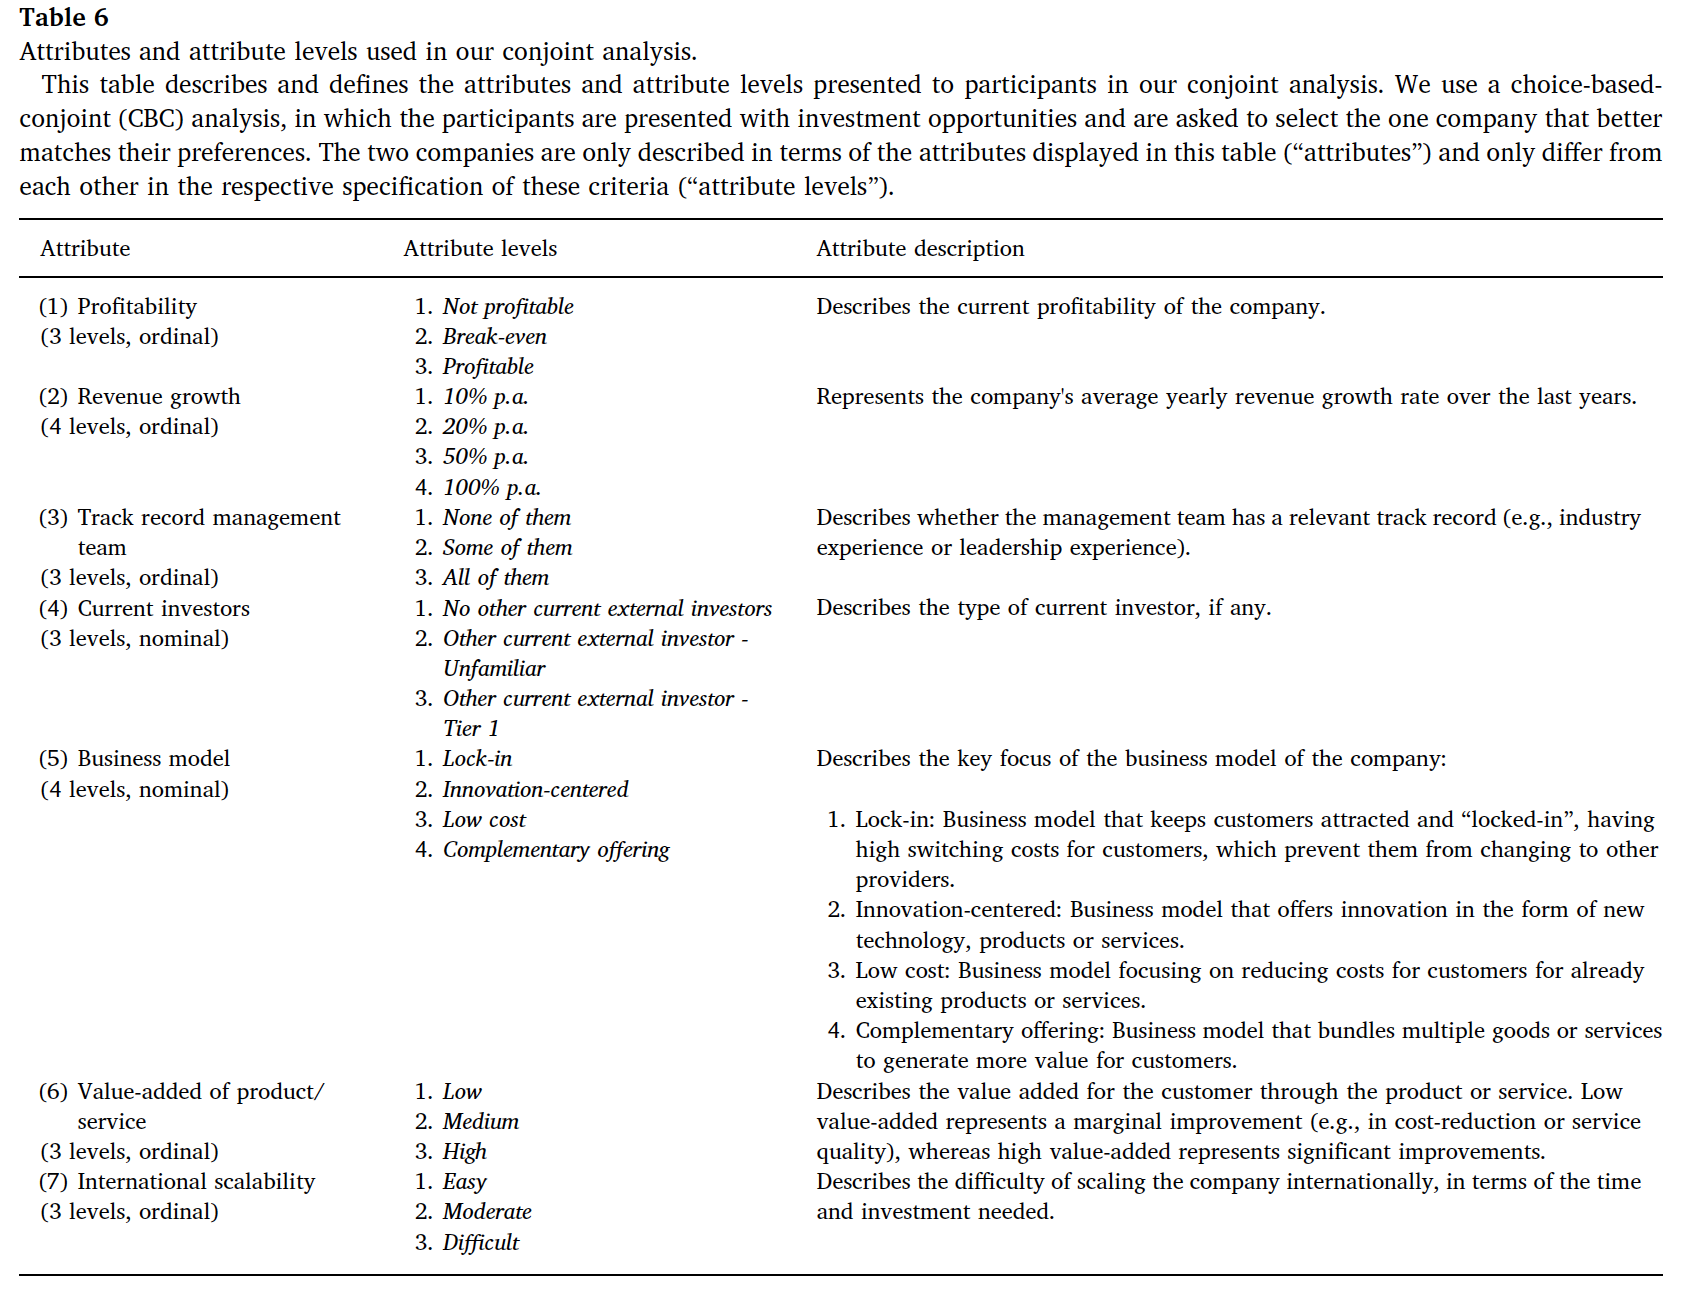
\includegraphics[width=\textwidth]{variables.png}
    \caption{Investment criteria and attributes from Block et al (\citeyear{BLOCK2019329})}
    \label{fig:ica}
\end{figure}
\begin{landscape}
	\begin{table}[H]
		\centering
		\begin{tabular}{|c | c | c | c|} 
		 \hline
		 Criteria & Relative Importance & Rank & Variables \\ 
				   & (Attributes,\%) 	& (\#) & \\ [0.5ex] 
		 \hline\hline
		 Revenue Growth & 23.4 & 1 & Revenue Growth (t-1, t-3, t-5) \\ 
		 				&  	   &   & 10\%, 20\%, 50\%, 100\% (p.a) \\ 
		 \hline
		 Value-added (Product/Service)& 20.4 & 2 & Low (1), Med (2), High (3) \\
		 \hline
		 Management Team Track Record& 15.7 & 3 & None (1), Some (2) , All (3) \\
		 \hline
		 International Scalability & 13.0  & 4 & Easy (1), Moderate (2), Difficult (3) \\
		 \hline
		 Profitability & 11.8 & 5 & EBITDA, EBIT, NOPAT, ROA, ROE (\$) \\ 
						 &      &   & Not profitable (1), Breakeven (2), Profitable (3) \\
		 \hline
		 Business Model & 8.3 & 6 & Lock in (1), Innovation-centered (2), Low Cost (3), Complimentary Offering (4) \\
		 \hline
		 Current Investors  & 7.3 & 7 & No Other Current External Investors (1),   \\ 
		 &  &  & Other Current Investors - Unfamiliar (2)\\
		 &  &  & Other Current Investors - Tier 1 (3)\\ [1ex]
		 \hline
		\end{tabular}
		\caption{Variables mapping investment criteria}
		\label{table:1}
		\end{table}
\subsection{Research Timetable}\label{RT}
This section of the appendix displays the proposed timeline for the research proposal.
The timetable displays the implementation of the proposal's methodology through time.
\begin{figure}[H]
    \centering
    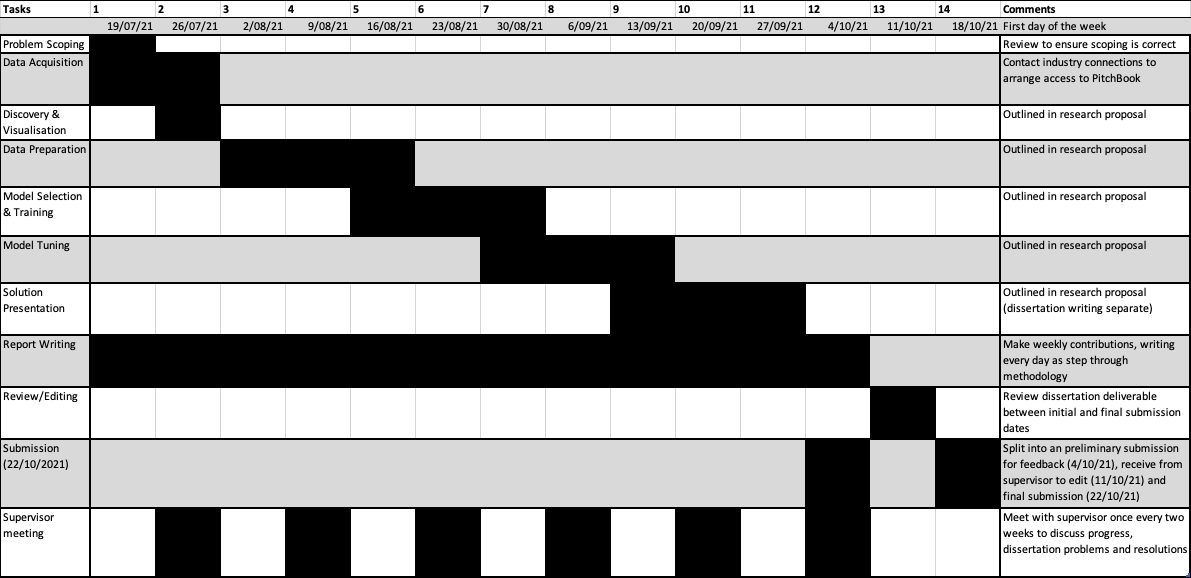
\includegraphics[width=1.5\textwidth]{rt.png}
    \caption{Research Timetable}
    \label{fig:rt}
\end{figure}
% \subsubsection{Research Overviews}
% Table \ref{table:PEF} outlines Private Equity-related literature by focus.
% Table \ref{table:PEDJ} outlines Private Equity-related literature by discipline and journal.
% \begin{table}[h!]
% \centering
% \begin{tabular}{c c c c c c c c } 
%  \hline
%  Source & Sample & Location & Firm Type & Data Source & Independent variable & Dependent Variables & Key Theoretical Findings\\ [0.5ex] 
%  \hline\hline
%  [X] &  [X] &  [X] &  [X] &  [X] &  [X] &  [X] &  [X]\\
%  \hline
%  [X] &  [X] &  [X] &  [X] &  [X] &  [X] &  [X] &  [X]\\ [1ex] 
%  \hline
% \end{tabular}
% \caption{Private Equity Research by Focus}
% \label{table:PEF}
% \end{table}
% \begin{table}[h!]
% 	\centering
% 	\begin{tabular}{||c | c | c | c | c | c | c | c ||} 
% 	 \hline
% 	 Source & Sample & Location & Firm Type & Data Source & Independent variable & Dependent Variables & Key Theoretical Findings\\ [0.5ex] 
% 	 \hline\hline
% 	 [X] &  [X] &  [X] &  [X] &  [X] &  [X] &  [X] &  [X]\\
% 	 \hline
% 	 [X] &  [X] &  [X] &  [X] &  [X] &  [X] &  [X] &  [X]\\ [1ex] 
% 	 \hline
% 	\end{tabular}
% 	\caption{Private Equity Research by Discipline and Journal}
% 	\label{table:PEDJ}
% 	\end{table}
\end{landscape}
\end{document}